
O motor de passo híbrido pode ser analisado de forma linear e não-linear. É apresentado o modelo dinâmico de acordo com a figura \ref{fig:fig1} por apresentar características em regime transitório e estacionário . O circuito equivalente é construído supondo que o circuito magnético é linear (não saturado) e a indutância mútua entre as fases é desconsiderada.

\begin{figure}[H]
	\centering
	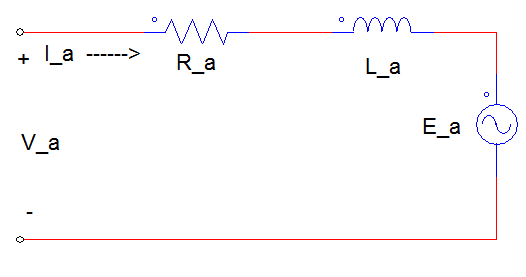
\includegraphics[scale=.42]{Images/graficofasea.PNG}
	\caption{ Circuito equivalente da bobina A}
	\label{fig:fig1}
\end{figure}

No modelo, $R_a$ e $L_a(\theta)$ representa respectivamente a resistência e a indutância da fase A do enrolamento. O enrolamento varia a indutância em função da posição do rotor.

\begin{eqnarray}
	\label{eq:eq1a}
	L_a(\theta) = L_0 + L_1\cos(\rho \theta)
\end{eqnarray}

onde $L_0$ é a indutância média, $L_1$ é a variação máxima da indutância e $\rho$ é o número de dentes do rotor.

Note que a posição de referência ($\theta = 0$), é quando o dente do rotor esta completamente alinhado com o polo do eixo A, então o enrolamento da fase A terá a indutância máxima.

Este modelo $R_a$ e $L_a$ representa respectivamente a resistência e indutância da fase A. Devido ao tamanho do entreferro, a indução dos enrolamentos do motor de passo híbrido pode ser considerado independente da posição do rotor. No caso de um motor de duas fases a tensão $E_a$ representa a FEM induzida na bobina A é uma função senoidal da posição do rotor

\begin{eqnarray}
	\label{eq:eq2a}
	E_a = \omega \rho \psi_m \sin(\rho \theta)
\end{eqnarray}

similar a FEM induzida pela bobina B, que é dado por

\begin{eqnarray}
		\label{eq:eq3a}
		E_b = \omega \rho \psi_m \sin(\rho \theta - \lambda)
\end{eqnarray}
onde
\begin{itemize}
	\item $\rho$ - número de dentes do rotor; \\
	\item $\psi_m$ - máximo fluxo concatenado; \\
	\item $\theta$ - posição angular do rotor; \\
	\item $\lambda$ - angulo de fase; \\
\end{itemize}

No caso de duas fases do estator, $\lambda = \frac{\pi}{2}$ e a equação de $E_b$ é modificado como se segue a equação (\ref{eq:eq4a})

\begin{eqnarray}
		\label{eq:eq4a}
		E_b = \omega \rho \psi_m \cos(\rho \theta )
\end{eqnarray}

De acordo com a análise da figura \ref{fig:fig1} e as equações (\ref{eq:eq1a}), (\ref{eq:eq2a}) e (\ref{eq:eq4a}), as equações das correntes são na forma de

\begin{eqnarray}
	\label{eq:eq5a}
	\frac{d i_A(t)}{dt} = \frac{1}{L_a}\left(V_A - Ri_A(t) + \omega(t) \rho \psi_m \sin(\rho \theta) \right) \\
	\label{eq:eq5b}
	\frac{d i_B(t)}{dt} = \frac{1}{L_b}\left(V_B - Ri_B(t) - \omega(t) \rho \psi_m \cos(\rho \theta) \right) 
\end{eqnarray}

onde
\begin{itemize}
	\item $V_A,\ V_B$ - tensões de fase; \\
	\item $R$ - resistência de fase do enrolamento; \\
	\item $i_A,\ i_B$ - correntes de fase;\\
\end{itemize}

O torque eletromagnético é formado pelas componentes do torque gerado referente a cada fase como segue nas equações (\ref{eq:eq6a}), (\ref{eq:eq6b})
\begin{eqnarray}
\label{eq:eq6a}
T_A = i_A \rho \psi_m \sin(\rho \theta)\\
\label{eq:eq6b}
T_B = i_B \rho \psi_m \cos(\rho \theta) 
\end{eqnarray}

Se o estator e o rotor tem dentes, o torque eletromagnético é complementado pela componente de torque devido a relutância gerado pela saliências do endentamento, chamado de torque de retenção (\textit{detent torque}) ou torque endentação, $T_d$ possui a equação (\ref{eq:eq7a})

\begin{eqnarray}
\label{eq:eq7a}
T_d = T_{d}^{max}\sin(2 \rho \theta)
\end{eqnarray}

O torque eletromagnético produzido por motor de passo híbrido de duas fases é igual ao somatório resultante da interação entre as correntes das duas fases além do fluxo magnético formado pelos ímãs juntamente com o torque de endentação

\begin{eqnarray}
	\label{eq:eq8a}
	T_e = - \rho \psi_m i_A \sin(\rho \theta) - \rho \psi_m i_B \cos(\rho \theta ) - T_d
\end{eqnarray}

O movimento do rotor é descrito pela equação (\ref{eq:eq9a}) de rotação do movimento, o que leva em conta a soma de inércia do rotor, torque de carga, torque eletromagnético e o torque de atrito viscoso.

\begin{eqnarray}
\label{eq:eq9a}
j\frac{d\omega(t)}{dt} = T_e(t) - T_L - B\omega(t)
\end{eqnarray}

Substituindo a equação (\ref{eq:eq8a}) em (\ref{eq:eq9a}) obtemos a equação (\ref{eq:eq10a}).

\tiny

\begin{eqnarray}
\label{eq:eq10a}
j\frac{d\omega(t)}{dt} = - \rho \psi_m i_A \sin(\rho \theta) - \rho \psi_m i_B \cos(\rho \theta ) )- T_{d}^{max}\sin(2 \rho \theta)  - T_L - B\omega(t)
\end{eqnarray}

\normalsize

Com as equações definidas, utiliza-se o modelo de espaço de estados para a resolução em tempo contínuo dadas as devidas considerações expostas anteriormente. 



\subsection{Simulação Computacional}

É possível simular o comportamento do motor por modelo genérico utilizando o $Simulink^\circledR$ conforme apresentado na figura \ref{fig:fig2}.

\begin{figure}[H]
	\centering
	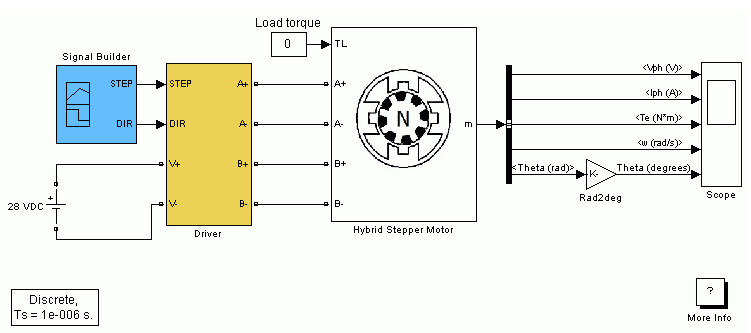
\includegraphics[scale=.42]{Images/modeloEE_HSM.PNG}
	\caption{ Modelo Genérico do Motor de Passo Híbrido - $Simulink^{\circledR}$ }
	\label{fig:fig2}
\end{figure}

O bloco representando o motor oferecer 5 sinais de saída sendo eles:

\begin{itemize}
	\item Tensão de fase ($V_f$);
	\item Corrente de fase ($I_f$);
	\item Torque eletromagnético ($T_e$);
	\item Velocidade angular do rotor ($\omega$);
	\item Posição do rotor ($\theta$);
\end{itemize}

Os parâmetros usados no modelo de motor de passo são usualmente obtidos na folha de dados do fabricante. No caso onde os parâmetros não estão disponíveis, pode ser determinado através de medidas experimentais.

Os parâmetros encontrados na folha de dados são geralmente: números de fases, torque de rotor travado (\textit{holding torque), angulo de passo, tensão de fase, resistencia do enrolamento($R_a$), maxima indutância($L_1^{max},\ para\ \theta=0$), indutância média ($L_0$) e inércia do motor ($J$).

O máximo torque de retenção($T_d^{max}$) não é especificado. Este parâmetro pode assume-se ser entre $1\%-10\%$ do torque máximo de rotor travado.





As características relacionadas com motores que estão em movimento ou preste a começar são chamadas de características dinâmicas.

A característica \textbf{pull-in} de torque chamada alternativamente de \textbf{característica de partida} e refere-se ao intervalo do torque de carregamento o qual o motor pode partir e parar sem perder sincronismo para várias frequências de acionamento.
A característica \textbf{pull-out} de torque chamada alternativamente de \textbf{característica de taxa de variação de carga}.

Após a partida do motor por um driver especificando o modo de excitação delimitado por sua gama de valores de partida, a frequência de pulso é aumentada gradualmente. O motor inicialmente ficará sem sincronismo. A relação entre o torque de carga e o máximo pulso de frequência com qual o motor pode sincronizar é chamado de característica pull-out. A curva pull-out é afetado pelo circuito driver, acoplamento, instrumentos de medição e outras condições.

Vejamos algumas características:

\textbf{Máxima Frequência de Partida}: é definido como a máxima frequência de controle no qual o motor sem cargapode iniciar e parar sem perder passos.